\chapter{THE STANDARD MODEL} \label{sm}

The Standard Model (SM) of particle physics is an incredibly successful theory that correctly describes the physics of all known particles and forces that make up the universe, excluding gravity \cite{smconsistency}. The particles of the SM come in two types: fermions and bosons. Fermions are the spin $\frac{1}{2}$ particles and make up the different types of matter, and bosons are the integer spin particles responsible for the different forces. Electrons are the most familiar type of fermion, but there are more exotic kinds like the up and down quarks that make up protons and neutrons. Electrons combine with the quark based nuclei to make atoms and account for nearly all of the matter in our day to day experience, but there are actually many other fermions. In fact, there are three generations of quarks and leptons \footnote{Leptons are fermions like the electron that aren't quarks. The quarks interact with the strong force that binds nuclei together and the leptons do not.} with each generation heavier than the next. The up and down quarks are the first generation of quarks, charmed and strange are the next, and top and bottom are the third generation. For the leptons, the electron and electron neutrino are the first generation, the muon and muon neutrino are the second, and the tau and the tau neutrino the third. Each fermion also has a corresponding antiparticle. As an example, the positron is the antiparticle for the electron. 

\begin{figure}[h!]
  \centering
  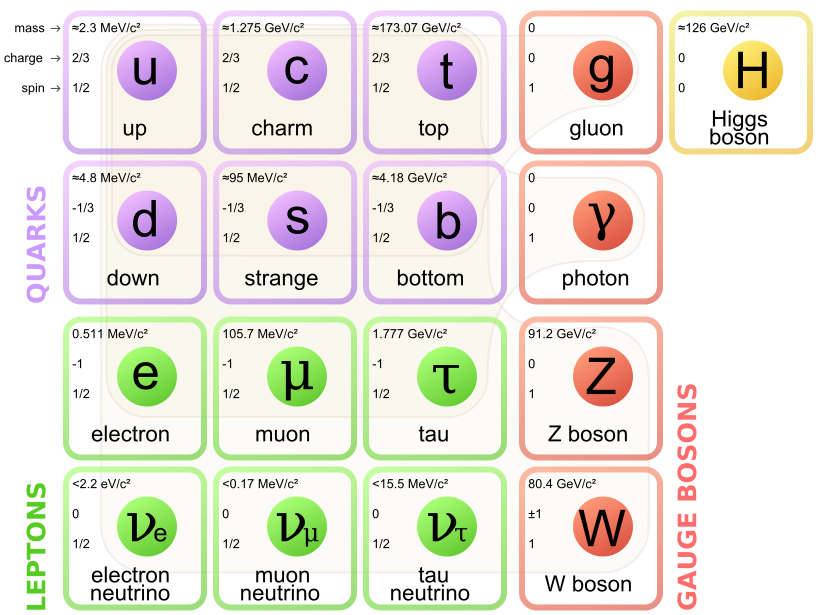
\includegraphics[width=4in]{images/Standard_Model_of_Elementary_Particles.png}
  \caption
   {The Standard Model Particles}
  \label{fig:smtable}
\end{figure}

The universe would be pretty boring if particles couldn't interact to form more complex objects like atoms, molecules, and even people. Luckily the different forces exist as well, and these forces are described by the spin 1 bosons. Fermions attract and repel by exchanging bosons, which is why the bosons are often called force carriers. The force mediating bosons are the gluons, photons, and the W and Z particles. Gluons mediate the strong force, photons the electromagnetic force, and the W and Z bosons mediate the weak force. Every force has an associated charge: particles with electric charge can interact through the electromagnetic force, those with color charge may interact via the strong force, and those with isospin may interact through the weak force. The fundamental forces and particles interact to make the familiar composite objects that surround us in our daily lives. The strong force binds quarks to form protons and neutrons, and even binds the protons and neutrons together to form nuclei, and the electromagnetic force binds electrons and nuclei to form atoms. The size of the composite objects gives an idea of the relative strength of the forces. A proton is ~$10^{-15}$ meters in size while an atom is ~$10^{-10}$ meters and a solar system is ~$10^{12}$ meters. The more tightly bound the stronger the force. In fact the ratio of the strength of the forces is like so 1:$10^{-3}$:$10^{-16}$:$10^{-41}$, strong : electromagnetic : weak :gravitational \footnote{Gravity is just included for perspective. The Standard Model does not describe this force and reconciling gravity with quantum mechanics is an open problem.}. 

Of all the particles predicted by the SM, only the Higgs boson remains to be found. The Higgs is the only spin 0 particle of the SM, and plays a special role. As the universe cooled from the Big Bang the Higgs field went through a phase transition and settled into a nonzero ground state forming a condensate. The potential energy from the interactions with this nonzero ground state give the massive fundamental particles their mass. With such a large role in the SM, finding this particle or a BSM Higgs has been a huge priority for the CMS collaboration \cite{tdr}. In 2012 a Higgs particle with a mass of 125 GeV was found and to date remains consistent with the Standard Model. However, the properties need to be investigated further before declaring the discovered Higgs the Higgs of the Standard Model. 

In order to lay out the Standard Model in mathematical terms, a bunch of background information needs to be covered, and since the Standard Model is described by Quantum Field Theory (QFT), the mathematical formulation of QFT will be covered first. After developing the necessary mathematical formalism, the Standard Model and the Higgs mechanism will be derived and explained. Afterwards the experimental search for Higgs to dimuons will be described.

In this dissertation $\hbar$ and the speed of light, c, are set to 1. Moreover, 0,1,2,3 and t,x,y,z are used interchangeably to label the components of a four vector. When relevant 0 represents time and 1,2,3 represent x,y,z respectively. Einstein summation notation is used indicating that repeated indices are summed over, so $x_ix_i y_jy_j$ is shorthand for $\sum_i\sum_j x_ix_i y_jy_j$. Repeated Greek indices assume sums over all four space and time components, while repeated Roman indices assume sums over only the spatial components. 

%%%%%%%%%%%%%%%%%%%%%%%%%%%%%%%%%%%%%%%%%%%%%%%%%%%%%%%%%%%%%%%%%%%%%%%%%%%

\section{Quantum Field Theory}


The mathematical framework used to describe the physics of the SM as well as other Beyond Standard Model (BSM) field theories is called Quantum Field Theory (QFT). QFT enables the predictions of different measurable probabilities. One of the most important is the probability for a set of particles to come out of a collision of an initial set of particles. Another important one is the probability for a single particle to decay into another set of particles. These probabilities are encompassed in the cross sections and branching fractions. For example, the theory of the SM predicts the cross section for two protons to collide and create a Higgs. As another example, the SM also predicts the branching fraction for a Z boson to decay into to two muons. These probabilities can be measured simply by colliding particles and counting the outcomes which in turn means that the theory can be tested. In fact, any QFT model can be tested in this manner. Quantum Field Theory is written down in terms of a Lagrangian, and the math for the various predictions follows from there, but first a brief aside about particles. 

\subsection{Particles, Symmetries, and Labels}

Since QFT makes quantitative predictions in terms of particle collisions and particle decays it's interesting to contemplate what a particle really is. Consider an observer in a frame x with particle p and an observer in another frame x'. If the observer in x' can't identify particle p as well then it doesn't make sense to call p a particle. More concretely, consider a world where in frame x an observer sees a neatly stacked deck of cards, but in x' the observer sees the cards scattered all over the place. Calling the deck of cards a particle doesn't really make sense. On the other hand, both parties can still agree on the individual cards which kept the same suit and value. The suit and value are conserved quantities identifiable between frames. If the two observers get together later and compare notes they can see what happened to each card upon transforming from x to x' and work out a set of rules. The king of hearts may do one thing and the 10 of clubs another. They can then add the different forces into play repeat the process and compare again. Figuring this all out allows the two to determine the laws of physics for the fundamental pieces called particles.       

This idea leads to Wigner's view: a particle is an object with conserved quantities that observers can agree on between frames. In our universe these labels are the mass, charge, spin, color, and isospin, with each label attached to a specific symmetry or group of symmetries. And because different observers can agree on these quantities they can compare notes and work out the laws of physics for the different types of particles. The deep connection between conserved quantities, symmetries, and labels for particles will be seen later. For now the focus is to work out laws that people in different frames can confirm, and this is where the Lagrangian formalism comes into play. 

\subsection{The Lagrangian Formalism}

The Lagrangian formalism is a mathematical device that allows physicists to describe the evolution of a physical system over time, and it's within this formalism that QFT can be built. But before building the full mathematics of QFT, a simple example describing the free Newtonian particle is covered. The Newtonian example serves to illuminate the fact that the laws of physics are indistinguishable in different inertial frames. Moving to the full relativistic theory reveals that the symmetry goes deeper. Investigating the symmetries of the relativistic theory end up leading the way to QFT, a relativistic description of quantum mechanics.

So let's get into the framework. The goal of physics is to describe how a physical system evolves over time, and this evolution is usually given by some differential equation describing the state the system will take in the next interval of time given the current time. Moving from state to state from one interval of time to the next, the system traces out a path in some abstract space of possible states. As a concrete example, the differential equations describing the motion of a Newtonian particle determine the position and velocity of the particle at the next instant of time based upon the values in the previous instant of time. So how does one get the appropriate differential equation? At classical scales, nature tries to minimize the difference between the energy spent \footnote{Spent here just means used as kinetic energy.} and the energy available to spend and it minimizes the action S. At the more fundamental level of quantum mechanics, all possible paths contribute with different phases, but those close to the minimum add constructively. As the action gets larger and the paths away from the minimum count less and less and the quantum rule agrees with the classical rule. The classical case is analyzed first to derive certain symmetries. In the equation below, L is the Lagrangian, T is the kinetic energy and U is the potential energy.     
\begin{equation}
S = \int L dt = \int T - U dt
\end{equation}

At an extremum of S, $\delta S$ = 0 if S is smooth: S must decrease, go through a slope of zero, and then increase (or vice versa). For a true extremum, $\delta S$ must be 0 in all directions. So to get the equations of motion vary the parameters of L and solve the system of equations for the values that yield zero change in the action.

\begin{equation}
\begin{split}
&\frac{\delta S}{\delta z_1} = \int L(z_1 + dz_1, z_2, ...)dt - \int L(z_1, z_2, ...)dt = 0 \\
&\frac{\delta S}{\delta z_2} = \int L(z_1, z_2 + dz_2, ...)dt - \int L(z_1, z_2, ...)dt = 0 \\
&...
\end{split}
\end{equation}

Following this process provides the Euler-Lagrange equations, describing how the parameters z evolve over time. The z's may be the position and velocity, or the quantum fields, or the temperature and volume or some other set of parameters that describe the system. The Lagrangian for a Newtonian free particle in one dimension is pretty simple and gets the point across. 

\begin{equation}
S = \frac{1}{2} \int m\dot{x}^2 dt
\end{equation}

If the action is at an extremum, perturbing the path x(t) by adding the infinitesimal $\epsilon$(t) leaves the action unchanged.

\begin{equation}
S' = \frac{1}{2} \int m(\dot{x} + \dot{\epsilon})^2 dt = \frac{1}{2} \int m(\dot{x}^2 + 2\dot{x}\dot{\epsilon} + \dot{\epsilon}^2) dt =  
\frac{1}{2} \int m(\dot{x}^2 + 2\dot{x}d\dot{x}) dt 
\end{equation}

\begin{equation}
\delta S = S' - S = 0 = \frac{1}{2} \int m(\dot{x}^2 + 2\dot{x}\dot{\epsilon}) dt - \frac{1}{2} \int m\dot{x}^2 dt = \int m\dot{x}\dot{\epsilon} dt
\end{equation}

Since x(t) is fixed at the boundaries of the integral, $\epsilon$ must be zero at $t_o$ and $t_f$, so integrating by parts yields the following equation. 

\begin{equation}
\delta S = 0 = \epsilon(t_f) \dot{x}(t_f)  - \epsilon(t_o) \dot{x}(t_o) + \int m\ddot{x} \epsilon dt  = 
0\dot{x}(t_f)  - 0\dot{x}(t_o) + \int m\ddot{x} \epsilon dt = \int m\ddot{x} \epsilon dt
\end{equation}

And this equation must be zero for any infinitesimal deviation $\epsilon$.

\begin{equation}
\delta S = 0 \rightarrow m\ddot{x} = 0
\end{equation}

So a free particle keeps the same velocity over time. Note that a Newtonian boost by constant velocity $v \rightarrow v' = v + u$ \footnote{Renaming $\dot{x}$ as v.} leaves the equations of motion consistent. In the unprimed frame the particle has velocity v with 0 acceleration. In the primed frame the particle has velocity v + u with 0 acceleration. Both observers see the particle act as if there are zero forces.

\begin{equation}
S = \frac{1}{2} \int m(v + u)^2 dt  =  \frac{1}{2} \int m(v')^2 dt \rightarrow \delta S = 0 \rightarrow m\frac{d}{dt}(v+u) = m\frac{d}{dt}(v') = 0 
\end{equation}

If u is not constant but a function of time u(t) then the equations of motion do not describe the same time evolution.

\begin{equation}
m\frac{d}{dt}(v+u) = m\dot{v} + m\dot{u} = 0 \rightarrow \dot{v} = -\dot{u}
\end{equation}

In the case where u(t) depends upon time, the difference between the primed and unprimed frames' equations of motion is then $\delta F$.

\begin{equation}
\delta F = m\frac{d}{dt}(v+u) - m\frac{dv}{dt} = m\dot{v} + m\dot{u} - m\dot{v} = m\dot{u}
\end{equation}

In the unprimed frame, the particle identified by the mass moves with constant velocity, $\dot{v} = 0$. The observer in the primed frame looks at the particle with the same mass and sees it change velocity given by the equation $\dot{v} = -\dot{u}$. As an example, set v and $u, \dot{u}$ to zero for all times before t=0, and let $u, \dot{u}$ turn on after time 0. Both observers will agree that the particle is stationary up until time 0. After which, the observer in the primed frame will see the particle accelerate in strange ways. Meanwhile, the unprimed frame will continue to observe a stationary particle. 

In general, every inertial frame finds $\delta F = 0$ and every accelerating frame finds an extra force $\delta F$ unique to its acceleration. In this way no observer in an inertial frame can perform an experiment and determine which inertial frame he or she is in. On the other hand, each accelerating frame is identified by its $\delta F$.  Put another way, in every inertial frame a ball released at rest remains at rest. In an accelerating frame the ball will accelerate according to the motion of the frame $\delta F$ and this change in the laws of physics identifies the frame in a unique way. Conversely, the laws of physics remain the same boosting between inertial frames, and this invariance is a symmetry of physics. Of course this example is Newtonian and the correct way to boost is given by the Lorentz transformation from Special Relativity, but this gets the point across.

Delving further along the path of symmetry, the fundamental forces depend only on the distance from the charge and not the direction implying that rotations are also a symmetry. This can be seen by looking at the Lagrangian. 

\begin{equation}
L = \frac{1}{2} m\dot{\vec{x}}^2 - U((\vec{x} - \vec{x'})^2)
\end{equation}

Rotations leave dot products and consequently the magnitude of vectors unchanged so the Lagrangian is invariant under this transformation. Naturally if the Lagrangian is invariant the equations of motion will be as well.

\begin{equation}
m\frac{d\vec{v}}{dt} = \vec{\nabla} U
\end{equation}

In the equations of motion above, both sides are vectors and vectors transform the same way under rotations so the equations of motion are invariant. Note that in the case of rotations both the Lagrangian and the equations of motion are invariant. While for Newtonian boosts only the equations of motion were invariant. This is due to the fact that Newtonian mechanics is the low velocity limit of relativistic mechanics. In the theory of Special Relativity the action for a massive free particle is written like so.

\begin{equation}
S = \int \frac{m}{2}u^{\mu}u_{\mu}d\tau
\end{equation}

Just as rotations preserve the dot product, Lorentz transformations (boosts and rotations) preserve the four vector product. Insofar, both the relativistic Lagrangian and the resulting equations of motion remain invariant under a boost or rotation to a new inertial frame. Building a Lagrangian out of four vector products gaurantees that it will remain invariant under Lorentz transformations. However, four vectors aren't the most fundamental objects with invariant products. By studying the properties of the Lorentz group, it's possible to find even more fundamental building blocks called spinors.

\subsection{QFT From Symmetry}

The laws of physics are invariant under boosts and rotations, and the Lagrangian provides a mathematical framework for physical predictions. These facts together imply that there's a good shot at building a proper QFT by creating the appropriate invariant Lagrangian. Four vector products remain invariant under Lorentz transformations so they are a natural ingredient, but there are other mathematical objects that could be used as well. In this vein, the symmetries under rotations and boosts are investigated in order to look for other building blocks. The goal is to find three different representations of the Lorentz group and use one representation for scalar spin 0 particles, another for the spin $\frac{1}{2}$ fermions, and another for the spin 1 bosons.

\subsubsection{Rotations}

Rotations in three dimensions are described by the SO(3) group. Rotations preserve the lengths of vectors and the angles between them, which means that dot products between vectors remain invariant as well. In three dimensions one can rotate about any of the three axes. The rotations about the x, y, and z axes may be characterized by the matrices below.

\begin{equation}
R_x = 
\begin{pmatrix}
1 & 0 & 0 \\
0 & \cos\theta_x & -\sin\theta_x \\
0 & \sin\theta_x & \cos\theta_x \\
\end{pmatrix}
\end{equation}

\begin{equation}
R_y = 
\begin{pmatrix}
\cos\theta_y & 0 & \sin\theta_y \\
0 & 1 & 0 \\
-\sin\theta_y & 0 & \cos\theta_y \\
\end{pmatrix}
\end{equation}

\begin{equation}
R_z = 
\begin{pmatrix}
\cos\theta_z & -\sin\theta_z & 0 \\
\sin\theta_z & \cos\theta_z & 0 \\
0 & 0 & 1 \\
\end{pmatrix}
\end{equation}

These rotations may be built up from repeated rotations by an infinitesimally small angle $d\theta$. The matrices characterizing an infinitesimal rotation are given by taking the limit as $\theta$ goes to zero.

\begin{equation}
dR_x = 
\begin{pmatrix}
1 & 0 & 0 \\
0 & 1 & -d\theta_x \\
0 & d\theta_x & 1 \\
\end{pmatrix}
= 1 - id\theta_x
\begin{pmatrix}
0 & 0 & 0 \\
0 & 0 & -i \\
0 & i & 0 \\
\end{pmatrix}
= 1 - id\theta_x J_x
\end{equation}

\begin{equation}
dR_y = 
\begin{pmatrix}
1 & 0 & d\theta_y \\
0 & 1 & 0 \\
-d\theta_y & 0 & 1 \\
\end{pmatrix}
= 1 - id\theta_y
\begin{pmatrix}
0 & 0 & i \\
0 & 0 & 0 \\
-i & 0 & 0 \\
\end{pmatrix}
= 1 - id\theta_y J_y
\end{equation}

\begin{equation}
dR_z = 
\begin{pmatrix}
1 & -d\theta_z & 0 \\
d\theta_z & 1 & 0 \\
0 & 0 & 1 \\
\end{pmatrix}
= 1 - id\theta_z 
\begin{pmatrix}
0 & -i & 0 \\
i & 0 & 0 \\
0 & 0 & 0 \\
\end{pmatrix}
= 1 - id\theta_z J_z
\end{equation}

Repeating an infinitesimal rotation many times builds the finite rotation, and in this way, the J matrices generate rotations along their respective axes.  As such, they are aptly referred to as the generators of the group. Doing some algebra reveals this to be the case. This point is confirmed below.

\begin{equation}
R = (1 - i\frac{\theta}{N} J)^{N} = 1 + (-id\theta J) + \frac{1}{2!}(-id\theta J)^2 + \frac{1}{3!}(-id\theta J)^3 + ... = e^{-i\theta J} 
\end{equation}

Notice that even powers of J yield $J^2$ and that odd powers of J return J.

\begin{equation}
  = 1 - J^2 + J^2(1 + \frac{i^2}{2!} d\theta^2 + \frac{i^4}{4!} d\theta^4 + ...) - iJ(d\theta + \frac{i^2}{3!}d\theta^3 + \frac{i^4}{5!}d\theta^5 + ...) 
  = (1-J^2) + J^2 \cos\theta - iJ\sin\theta
\end{equation}

Plugging in $J_z$ reveals that this process does in fact rebuild the rotation matrix $R_z$.

\begin{equation}
\begin{split}
R_z &= 
(\begin{pmatrix}
1 & 0 & 0 \\
0 & 1 & 0 \\
0 & 0 & 1 \\
\end{pmatrix}
-
\begin{pmatrix}
1 & 0 & 0 \\
0 & 1 & 0 \\
0 & 0 & 0 \\
\end{pmatrix})
+
\begin{pmatrix}
1 & 0 & 0 \\
0 & 1 & 0 \\
0 & 0 & 0 \\
\end{pmatrix}
\cos\theta_z
+
\begin{pmatrix}
0 & -1 & 0 \\
1 & 0 & 0 \\
0 & 0 & 0 \\
\end{pmatrix}
\sin\theta_z
\\ &=
\begin{pmatrix}
\cos\theta_z & -\sin\theta_z & 0 \\
\sin\theta_z & \cos\theta_z & 0 \\
0 & 0 & 1 \\
\end{pmatrix}
\end{split}
\end{equation}

Similarly, the other generators rebuild their respective rotation matrices. The generators of the group are actually more fundamental than the rotation matrices. The multiplication table for the generators describes the algebra of the group, which describes the behavior of rotations at a local level. In fact the SO(3) rotation matrices are just one of the groups with this local algebra, and a specific group obeying the local algebra is analagous to a specific solution of a differential equation: each solution has a different global behavior yet each obeys the same physics. Moreover the multiplication table can be specified without declaring any particular representation for the generators. 

\begin{equation}
\begin{split}
&J_x*J_y = iJ_z  + J_y*J_x \\
&J_y*J_z = iJ_x  + J_z*J_y \\
&J_z*J_x = iJ_y  + J_x*J_z \\
\end{split}
\end{equation}

The multiplication table can be specified in a more compact notation using the commutator \footnote{The Lie Bracket defines the multiplication for a Lie Algebra and this reduces to the commutator for Lie groups of matrices like SO(3). Notice that using the commutator below returns another member of the group and thus the group is closed under commutation.}, $[a,b] = ab - ba$, and the antisymmetric tensor $\epsilon$.
\begin{equation}
[J_k, J_l] = i\epsilon_{klm}J_m
\end{equation}

Finding 3x3 generators that obey the algebra and then repeatedly applying the infinitesimal transormations builds the SO(3) rotation group. The group acts on real 3x1 objects called vectors, and these 3x1 vectors are a suitable candidate for a Newtonian Lagrangian. Finding another representation obeying this algebra will provide a more fundamental ingredient for the Lagrangian and allow the construction of a proper QFT. Similar to the way real numbers are built from the squares of imaginary numbers, vectors are built from spinors. 

Looking for the lowest order nontrivial nxn matrices satisfying the algebra gives the 2x2 Pauli matrices. The 1x1 matrices are the trival solution: 1x1 matrices are simply scalar complex numbers, which commute and therefore fail to satisfy the algebra unless all of the J matrices are 0. The objects these 1x1 operators act on are 1x1 numbers called scalars which remain invariant under rotations and correspond to spin 0. The solution for the 2x2 case, the Pauli matrices are given by

\begin{equation}
\sigma_x = 
\begin{pmatrix}
0 & 1 \\
1 & 0 \\
\end{pmatrix},
\sigma_y = 
\begin{pmatrix}
0 & -i \\
i & 0 \\
\end{pmatrix},
\sigma_y = 
\begin{pmatrix}
1 & 0 \\
0 & -1 \\
\end{pmatrix}
\end{equation}

However, plugging these into the commutator reveals a factor of two difference.

\begin{equation}
[\sigma_k, \sigma_l] = 2i\epsilon_{klm}\sigma_m
\end{equation}

Defining $J_k = \frac{1}{2} \sigma_k$ fixes this. These matrices act on an array of 2x1 complex numbers called spinors, and this new rotation group is called SU(2). Note that by starting with vectors and analyzing the SO(3) rotation group along with its underlying algebra, new mathematical objects have been discovered. The 1x1 matrices satisfying the rotation algebra make up the spin 0 representation of SU(2), the complex 2x2 matrices acting on complex 2x1 objects satisfying the algebra make up the spin $\frac{1}{2}$ representation, and the complex 3x3 matrices acting on complex 3x1 objects satisfying the algebra make up the spin 1 representation. The pattern continues on. There are in fact many representations of SU(2). It's now possible to use these representations to build rotationally invariant Lagrangians, using the 2x1 spinors of SU(2) to model fermions and the 3x1 representation to model bosons. While rotationally invariant Lagrangians are important for nonrelativistic theories, the real goal is to break down four vectors in the same way to find the most fundamental ingredients for relativistic Lagrangians. 

\begin{equation}
[J_k, J_l] = i\epsilon_{klm}J_m
\end{equation}

\subsubsection{The Lorentz Group}
Four vector products are invariant with regards to rotations and boosts. This statement is defined by the mathematical equation below, where the $\Lambda$ matrices represent the rotation/boost matrices of the Lorentz Group \footnote{The Lorentz group dealt with here is the proper orthochronous Lorentz Group SO(1,3).} and the $\eta$ matrix is the Minkowski metric $\left( \begin{smallmatrix} 1 & 0 & 0 & 0 \\ 0 & -1 & 0 & 0 \\ 0 & 0 & -1 & 0 \\ 0 & 0 & 0 & -1 \\ \end{smallmatrix} \right)$.

\begin{equation}
x'_{\mu} x'^{\mu} = x_{\mu} x^{\mu} \rightarrow \eta_{\sigma\rho} \Lambda^{\sigma}_{\mu}  \Lambda^{\rho}_{\nu} x^{\mu} x^{\nu} = \eta_{\mu\nu} x^{\mu} x^{\nu}
\rightarrow \eta_{\sigma\rho} \Lambda^{\sigma}_{\mu}  \Lambda^{\rho}_{\nu} = \eta_{\mu\nu}
\end{equation}

In this 3 + 1 dimensional space the rotations and their corresponding generators are now given by the following R and J matrices, where the R matrices satisfy the equation above.

\begin{equation}
R_x = 
\begin{pmatrix}
1 & 0 & 0 & 0\\
0 & 1 & 0 & 0 \\
0 & 0 & \cos\theta_x & -\sin\theta_x \\
0 & 0 & \sin\theta_x & \cos\theta_x \\
\end{pmatrix},
J_x = 
\begin{pmatrix}
0 & 0 & 0 & 0\\
0 & 0 & 0 & 0 \\
0 & 0 & 0 & -i \\
0 & 0 & i & 0 \\
\end{pmatrix}
\end{equation}

\begin{equation}
R_y = 
\begin{pmatrix}
1 & 0 & 0 & 0\\
0 & \cos\theta_y & 0 & \sin\theta_y \\
0 & 0 & 1 & 0 \\
0 & -\sin\theta_y & 0 & \cos\theta_y \\
\end{pmatrix},
J_y = 
\begin{pmatrix}
0 & 0 & 0 & 0\\
0 & 0 & 0 & i \\
0 & 0 & 0 & 0 \\
0 & -i & 0 & 0 \\
\end{pmatrix}
\end{equation}

\begin{equation}
R_z = 
\begin{pmatrix}
1 & 0 & 0 & 0\\
0 & \cos\theta_z & -\sin\theta_z & 0 \\
0 & \sin\theta_z & \cos\theta_z & 0 \\
0 & 0 & 0 & 1 \\
\end{pmatrix},
J_z = 
\begin{pmatrix}
0 & 0 & 0 & 0\\
0 & 0 & -i & 0 \\
0 & i & 0 & 0 \\
0 & 0 & 0 & 0 \\
\end{pmatrix}
\end{equation}

And the boosts are given by the following B matrices. These also leave the four vector product invariant.

\begin{equation}
B_x = 
\begin{pmatrix}
\cosh\omega_x & \sinh\omega_x & 0 & 0 \\
\sinh\omega_x & \cosh\omega_x & 0 & 0 \\
0 & 0 & 1 & 0 \\
0 & 0 & 0 & 1 \\
\end{pmatrix}
\end{equation}

\begin{equation}
B_y = 
\begin{pmatrix}
\cosh\omega_y & 0 & \sinh\omega_y & 0 \\
0 & 1 & 0 & 0 \\
\sinh\omega_y & 0 & \cosh\omega_y & 0 \\
0 & 0 & 0 & 1 \\
\end{pmatrix}
\end{equation}

\begin{equation}
B_z = 
\begin{pmatrix}
\cosh\omega_z & 0 & 0 & \sinh\omega_z \\
0 & 1 & 0 & 0 \\
0 & 0 & 1 & 0 \\
\sinh\omega_z & 0 & 0 & \cosh\omega_z \\
\end{pmatrix}
\end{equation}

Looking at the differential boosts yields the generators K.

\begin{equation}
dB_x = 
\begin{pmatrix}
1 & d\omega_x & 0 & 0 \\
d\omega_x & 1 & 0 & 0 \\
0 & 0 & 1 & 0 \\
0 & 0 & 0 & 1 \\
\end{pmatrix}
= 1 + d\omega_x 
\begin{pmatrix}
0 & 1 & 0 & 0 \\
1 & 0 & 0 & 0 \\
0 & 0 & 0 & 0 \\
0 & 0 & 0 & 0 \\
\end{pmatrix}
= 1 + d\omega_x K_x
\end{equation}

\begin{equation}
dB_y = 
\begin{pmatrix}
1 & 0 & d\omega_y & 0 \\
0 & 1 & 0 & 0 \\
d\omega_y & 0 & 1 & 0 \\
0 & 0 & 0 & 1 \\
\end{pmatrix}
= 1 + d\omega_y
\begin{pmatrix}
0 & 0 & 1 & 0 \\
0 & 0 & 0 & 0 \\
1 & 0 & 0 & 0 \\
0 & 0 & 0 & 0 \\
\end{pmatrix}
= 1 + d\omega_y K_y
\end{equation}

\begin{equation}
dB_z = 
\begin{pmatrix}
1 & 0 & 0 & d\omega_z \\
0 & 1 & 0 & 0 \\
0 & 0 & 1 & 0 \\
d\omega_z & 0 & 0 & 1 \\
\end{pmatrix}
= 1 + d\omega_z
\begin{pmatrix}
0 & 0 & 0 & 1 \\
0 & 0 & 0 & 0 \\
0 & 0 & 0 & 0 \\
1 & 0 & 0 & 0 \\
\end{pmatrix}
= 1 + d\omega_z K_z
\end{equation}

As before with the algebra for rotations in three dimensions the Lorentz algebra is defined by its multiplication table, but now there are rotations and boosts. The multiplication table is given by the commutation relations below, which can be confirmed by brute force computation.  

\begin{equation}
[J_i, J_j] = i\epsilon_{ijk}J_k
\end{equation}

\begin{equation}
[J_i, K_j] = i\epsilon_{ijk}K_k
\end{equation}

\begin{equation}
[K_i, K_j] = -i\epsilon_{ijk}J_k
\end{equation}

Notice that the commutator between J matrices returns another J matrix, but that the commutator between K matrices returns a J matrix. This means that the J operators form their own subgroup, but the K operators don't. On the other hand, mixing the Js and Ks up by defining the $Y^{\pm}$ operators allows the Lorentz algebra to be represented by two independent subgroups. 

\begin{equation}
Y^{\pm} = \frac{1}{2}(J_i \pm iK_i)
\end{equation}

\begin{equation}
[Y^{\pm}_i, Y^{\pm}_j] = i\epsilon_{ijk}Y^{\pm}_k
\end{equation}

\begin{equation}
[Y^{\pm}_i, Y^{\mp}_j] = 0
\end{equation}

Both of the Y groups have the same commutation relations as SU(2). In this way, the Lorentz algebra can be viewed as if two SU(2) rotation algebras have been glued together. This is similar to the way in which orthogonal basis vectors are stuck together to create a larger dimensional space. Now, in order to figure out how to use this space to build the appropriate Lagrangians, the individual subspaces must be investigated. So looking at $Y^{+}$ alone is akin to looking along the $Y^{+}$ axis by setting $Y^{-}$ to zero. Using $(y_+, y_-)$ to label the representation, the simplest nontrivial case along the $Y^{+}$ axis is spin $\frac{1}{2}$ x spin 0, given by $(\frac{1}{2}, 0)$.   

Using $Y_{i}^{-} = \frac{1}{2}(J_i - iK_i) = 0$ implies that $J_i = iK_i$, and since $Y_{i}^{+}$ is the 2x2 representation obeying the SU(2) algebra, $Y_{i}^{+} = \frac{\sigma_i}{2}$. Putting this together,

\begin{equation}
\begin{split}
J_i &= iK_i \\ 
&\rightarrow Y^+_i = \frac{1}{2}(J_i + iK_i) = \frac{\sigma_i}{2} = \frac{1}{2}(J_i + J_i) = J_i \\
&\rightarrow J_i = \frac{1}{2}\sigma_i \\
&\rightarrow K_i = \frac{-i\sigma_i}{2} \\
\end{split}
\end{equation} 
Finally, the finite Lorentz transformations for the $(\frac{1}{2}, 0)$ representation are given by 

\begin{equation}
R^{(L)} = e^{i\theta_i J_i} = e^{i\theta_i \frac{\sigma_i}{2}}   
\end{equation}

for rotations, and

\begin{equation}
B^{(L)} = e^{i\phi_i K_i} = e^{\phi_i \frac{\sigma_i}{2}}   
\end{equation}

for boosts. These act on 2x1 objects called left-chiral spinors, $\mathcal{L}$. A general Lorentz transformation on a left-chiral spinor can be written

\begin{equation}
\Lambda^{(L)} = e^{\frac{i}{2}\theta_i \sigma_i + \frac{1}{2}\phi_i \sigma_i}
\end{equation}.

Replacing $K_i$ with $-K_i$ takes $Y^+_i$ to $Y^-_i$, and gives the finite Lorentz transformations for the $(0, \frac{1}{2})$ representation 

\begin{equation}
R^{(R)} = e^{i\theta_i J_i} = e^{\frac{i}{2}\theta_i \sigma_i}   
\end{equation}

for rotations, and

\begin{equation}
B^{(R)} = e^{i\phi_i K_i} = e^{-\phi_i \frac{\sigma_i}{2}}   
\end{equation}

for boosts. These act on 2x1 objects called right-chiral spinors, $\mathcal{R}$. The general Lorentz transformation on a right-chiral spinor can be written

\begin{equation}
\Lambda^{(R)} = e^{\frac{i}{2}\theta_i \sigma_i - \frac{1}{2}\phi_i \sigma_i}
\end{equation}

Last but not least, rank 2 spinors are given by the $(\frac{1}{2}, \frac{1}{2})$ representation. This representation is a tensor combining two spinors via outer product, and as will be shown later, these objects are actually four vectors.

\begin{equation}
\alpha = \mathcal{L} \mathcal{R}^{T}
\end{equation}

In order to transform $\alpha$, both $\mathcal{L}$ and $\mathcal{R}$ must be transformed.

\begin{equation}
\alpha^{'} = \Lambda^{(L)} \mathcal{L} \mathcal{R}^T \Lambda^{(R)T} 
 = e^{\frac{i}{2}\theta_i \sigma_i + \frac{1}{2}\phi_i \sigma_i} \mathcal{L} \mathcal{R}^T e^{\frac{i}{2}\theta_i \sigma_i^T - \frac{1}{2}\phi_i \sigma_i^T} 
\end{equation}

However it would be nice if the transformation term on the right side was the Hermitian conjugate of the transformation on the left side. This would be the case if $\sigma_i^T$ was $-\sigma_i^{\dagger} = -(\sigma_i^{*})^{T}$, and this requires a transformation that turns $\sigma$ into $-\sigma^{*}$. So $\mathcal{R}$ is rearranged such that $\mathcal{R} \rightarrow \tilde{\mathcal{R}} = t\mathcal{R}$ where $t\sigma_i t^{-1} = -\sigma_i^{*}$. The matrix $t = \left( \begin{smallmatrix} 0 & -1 \\ 1 & 0 \\ \end{smallmatrix} \right)$ satisfies the requirements. This change of basis for $\mathcal{R}$ redefines $\alpha$,

\begin{equation}
\alpha = \mathcal{L}\tilde{\mathcal{R}}^T.
\end{equation}

Defined in this manner, the $(\frac{1}{2}, \frac{1}{2})$ representation now transforms like so,

\begin{equation}
\alpha^{'} = e^{\frac{i}{2}\theta_i \sigma_i + \frac{1}{2}\phi_i \sigma_i} 
\mathcal{L}\tilde{\mathcal{R}}^T e^{-\frac{i}{2}\theta_i \sigma_i^\dagger + \frac{1}{2}\phi_i \sigma_i^\dagger}.
\end{equation}

Considering the fact that $\sigma_i^\dagger = \sigma_i$, the transformation reduces further,

\begin{equation}
\alpha^{'} = e^{\frac{i}{2}\theta_i \sigma_i + \frac{1}{2}\phi_i \sigma_i} 
\alpha e^{-\frac{i}{2}\theta_i \sigma_i + \frac{1}{2}\phi_i \sigma_i}.
\end{equation}

A transformation of the form $M' = HMH^\dagger$ where H is a Hermitian matrix, preserves the Hermitivity of the matrix M. Namely, M' will be Hermitian if M is Hermitian, 

\begin{equation}
M^{'\dagger} = (HMH^\dagger)^\dagger = HM^\dagger H^\dagger = HMH^\dagger = M^{'}.
\end{equation}

On the other hand, M' will be anti-Hermitian if M is anti-Hermitian,

\begin{equation}
M^{'\dagger} = (HMH^\dagger)^\dagger = HM^\dagger H^\dagger = H(-M)H^\dagger = -HMH^\dagger = -M'.
\end{equation}

The transformation of the $(\frac{1}{2}, \frac{1}{2})$ object $\alpha$ is of this type. With this in mind, note that any complex matrix can be broken up into a Hermitian piece and an anti-Hermitian piece, and that these pieces remain independent under the $(\frac{1}{2}, \frac{1}{2})$ Lorentz transformations constructed here. Then note that a general complex 2x2 matrix has 8 free parameters, 4 from the Hermitian part and 4 from the anti-Hermitian part. Meanwhile, $\alpha$ has only 4, two from each spinor \footnote{A spinor has 2 complex components yielding 4 parameters. Two constraints reduce the number of free parameters to 2. One constraint requires a magnitude of 1, and the other requires that the overall phase doesn't matter.}. This means that $\alpha$ may be represented by the Hermitian space alone. An appropriate basis for this space is the collection of Pauli matrices plus the identity.

\begin{equation}
\sigma_0 =  
\begin{pmatrix}
1 & 0 \\
0 & 1 \\
\end{pmatrix}
\sigma_1 =  
\begin{pmatrix}
0 & 1 \\
1 & 0 \\
\end{pmatrix}
\sigma_2 = 
\begin{pmatrix}
0 & -i \\
i & 0 \\
\end{pmatrix}
\sigma_3 = 
\begin{pmatrix}
1 & 0 \\
0 & -1 \\
\end{pmatrix}
\end{equation}

Thus any $(\frac{1}{2}, \frac{1}{2})$ object $\alpha$ may be written in terms of its four independent parameters like so, 

\begin{equation}
\begin{split}
&\alpha = \alpha_0 \sigma_0 + \alpha_1 \sigma_1 + \alpha_2 \sigma_2 + \alpha_3 \sigma_3 \\
&\alpha = 
\begin{pmatrix}
\alpha_0 + \alpha_3 & \alpha_1 - i\alpha_2 \\
\alpha_1 + i\alpha_2 & \alpha_0 - \alpha_3 \\
\end{pmatrix}
\end{split}
\end{equation}

Boosting $\alpha$ along the z direction hints that the four components transform like a four vector.  

\begin{equation}
\alpha^{'} = e^{\frac{1}{2}\phi_3 \sigma_3} 
\begin{pmatrix}
\alpha_0 + \alpha_3 & \alpha_1 - i\alpha_2 \\
\alpha_1 + i\alpha_2 & \alpha_0 - \alpha_3 \\
\end{pmatrix}
e^{\frac{1}{2}\phi_3 \sigma_3}
\end{equation}

Exponentiating the $\sigma_3$ matrix and multiplying everything yields,

\begin{equation}
\begin{split}
\begin{pmatrix}
\alpha_0' + \alpha_3' & \alpha_1' - i\alpha_2' \\
\alpha_1' + i\alpha_2' & \alpha_0' - \alpha_3' \\
\end{pmatrix}
&=
\begin{pmatrix}
e^{\frac{1}{2}\phi_3} & 0 \\
0 & e^{-\frac{1}{2}\phi_3} \\
\end{pmatrix}
\begin{pmatrix}
\alpha_0 + \alpha_3 & \alpha_1 - i\alpha_2 \\
\alpha_1 + i\alpha_2 & \alpha_0 - \alpha_3 \\
\end{pmatrix}
\begin{pmatrix}
e^{\frac{1}{2}\phi_3} & 0 \\
0 & e^{-\frac{1}{2}\phi_3} \\
\end{pmatrix} \\
&=
\begin{pmatrix}
e^{\phi_3}(\alpha_0 + \alpha_3) & (\alpha_1 - i\alpha_2) \\
(\alpha_1 + i\alpha_2) & e^{-\phi_3}(\alpha_0 - \alpha_3) \\
\end{pmatrix}.
\end{split}
\end{equation}

Then solving the systems of equations makes the transformation clearer,

\begin{equation}
\begin{split}
&\alpha_1' = \alpha_1 \\
&\alpha_2' = \alpha_2 \\
&\alpha_0' = (\cosh\phi_3) \alpha_0 +  (\sinh\phi_3) \alpha_3 \\ 
&\alpha_3' = (\sinh\phi_3) \alpha_0 +  (\cosh\phi_3) \alpha_3. \\ 
\end{split}
\end{equation}

Finally the transformation can be written as a 4x4 matrix acting on the 4x1 four vector,

\begin{equation}
\alpha' = 
\begin{pmatrix}
\cosh\phi_3 & 0 & 0 & \sinh\phi_3 \\
0 & 1 & 0 & 0 \\
0 & 0 & 1 & 0 \\
\sinh\phi_3 & 0 & 0 & \cosh\phi_3 \\
\end{pmatrix}
\begin{pmatrix}
\alpha_0 \\
\alpha_1 \\
\alpha_2 \\
\alpha_3 \\
\end{pmatrix}
\end{equation}

The other transformations reproduce the usual 4x4 Lorentz transformations as well. In this way, four vectors are just rearranged versions of the $(\frac{1}{2}, \frac{1}{2})$ rank 2 spinors. Similar to the way complex numbers are the square root of real numbers, spinors are the square root of four vectors. In practice it's easier to work with 4 vectors as 4x1 column vectors, though one could use the $(\frac{1}{2}, \frac{1}{2})$ rank 2 spinor representation.  

\subsubsection{The Poincare Group and Particle Labels}

The Poincare group is the Lorentz Group plus translations. Physics experiments should be the same with a rotated apparatus, an apparatus moving at a different constant velocity, and also at another location. Adding translations to the group amounts to adding another the set of translation generators $P_i$. In the "Particles, Symmetries, and Labels" section the argument was made that particles are things that observers agree on between frames. Distinguishable particles have labels that remain invariant. A spin $\frac{1}{2}$ particle with mass m remains a spin $\frac{1}{2}$ particle with mass m for all observers. As it turns out these labels relate to different subspaces in the representation of the group.

Consider a group with certain generators. When the operators of the group are represented a certain way, say as some NxN matrices there is a likelihood that there are some invariant subspaces. As an example, a representation of a group may act on a 5 dimensional space spanned by vectors $e_1, e_2, e_3, e_4, e_5$. The group may always transform vectors in the $e_1, e_2, e_3$ subspace into one another, and those in $e_4, e_5$ into one another, but never mix up $e_1, e_2, e_3$ with $e_4, e_5$. In this example the 5x5 operators could be decomposed into a 3x3 operator acting only on the $e_1, e_2, e_3$ subspace and a 2x2 operator acting only on the $e_4, e_5$ subspace. Each 5x5 member of the group could be written as a block diagonal matrix with a 3x3 block and a 2x2 block. The same goes for the generators. Since these subspaces retain their identity under the transformations of the group\footnote{This assumes that the 3x3 and 2x2 pieces have no invariant subspaces besides themselves and 0.}, they may be considered different particles. The question is whether there are labels for the subspaces.  

Labels in physics need to be measurable, and by the current understanding of quantum mechanics these must be eigenvalues of Hermitian operators. The operators that label these subspaces are called the Casimir operators and must be built from the generators of the group. The operators should give the same values for $e_1, e_2, and e_3$ since they transform into one another and represent the same particle, which implies that the Casimir labeling operator must be proportional to the identity in that subspace. The same goes for the operator in the $e_4, e_5$ subspace. The Casimir operator for SU(2) is the $J^2$ operator which labels the spin of the particle. The Poincare group has two Casimir operators coresponding to two labels the mass, m, and the spin, j. Looking at the irreducible representations\footnote{This is the group theory term for the block diagonal pieces and the corresponding invariant subspaces. The irreducible representations, irreps, are those that can't be broken down in terms of smaller invariant subspaces and smaller block diagonal matrices. An arbitrary representation of the group is built from these irreps.} of the Poincare group, the mass and spin arise naturally as labels for particles. 

%Now the 5x5 group can be analyzed in terms of its separate 3x3 and 2x2 pieces. In group theory lingo these pieces are called the irreducible representations. This is the difference between a spin $\frac{3}{2}$ group and a group consisting of separate spin $\frac{1}{2}$ and spin 1 particles.

\subsubsection{Building the Lagrangian for a Free Scalar Particle}

Analyzing the symmetries of the SO(3) rotation group revealed the SU(2) group, the 2x2 complex Pauli matrices, and the complex 2x1 spinors. Analyzing the symmetries of the Lorentz group revealed the $(\frac{1}{2}, 0)$ left-chiral spinors, the $(0, \frac{1}{2})$ right chiral spinors, and the four vectors encoded in the $(\frac{1}{2}, \frac{1}{2})$ representation. Now, these pieces are put together to form relativistically invariant Lagrangians for free particles.  

The $(0,0)$ representation of the Lorentz group is a scalar, which means that it remains the same under Lorentz transformations. This representation is used for spin 0 particles. The equations of motion must relate the change in the scalar field $\Phi$ at one moment in space and time to the value of $\Phi$ at the next moment in space and time, so the Lagrangian must include both the field itself and the four vector derivative, $\partial_\mu$. Note that both Newton's equations of motion, $F=m\ddot{x}$, and the Schrodinger equation for the free particle, $i\partial_t\psi = \frac{1}{2m}(-i\partial_x)(-i\partial_x)\psi$\footnote{Here the one dimensional case is presented for simplicity} have at most second order derivatives. The same holds for Maxwell's equations of electromagnetism. Hence, as an assumption, the derivative term in the Lagrangian will be the lowest order possible. As a Lorentz invariant scalar, any power of $\Phi$ can be included. On the other hand, $\partial_\mu$ is a four vector, and must be paired with a $\partial^\mu$ to form the invariant four vector product. Cross terms between these invariant pieces are also invariant, but lead to feedback between the derivatives and the value of the function. This means that the derivatives $i\partial_t = E$ and $-i\partial_i = P_i$ will change over time, but E and $\vec{P}$ should remain constant for a free particle. The cross terms are thrown out to prevent this. The $\Phi$ terms with an order different than $\Phi^2$ cause the same problem, and these are thrown out too. All of these choices lead to the following action, 

\begin{equation}
S = \int d^4x \left(c_0 + c_1 \Phi^2  
+ c_2 \partial_\mu\Phi\partial^\mu\Phi + c_3 \partial_\mu \partial^\mu \Phi\right).
\end{equation}

Note that the $c_3$ term is a total derivative and by the divergence theorem depends only on the values at the boundary, which are fixed. This implies that the contribution to the action from the $c_3$ term is the same regardless of how $\Phi$ changes in the volume. Because the Euler-Lagrange equations depend only on the variation in the volume, this term cannot contribute to $\delta S$ and $c_3$ may be set to zero. The $c_0$ term is a more obvious constant and does not affect $\delta S$ either, so it may be set to zero as well. 

\begin{equation}
S = \int d^4x \left(c_1 \Phi^2 + c_2 \partial_\mu\Phi\partial^\mu\Phi\right)
\end{equation}

Finding $\Phi$ such that $\delta S = 0$ amounts to applying the Euler-Lagrange equations $\partial_\mu \frac{\partial L}{\partial\left(\partial_\mu\Phi\right)} = \frac{\partial L}{\partial \Phi}$. These yield 

\begin{equation}
\begin{split}
&2c_2\partial_\mu\partial^\mu\Phi = -2c_1\Phi \\ 
&\rightarrow (-E^2 + \vec{P}^2)\Phi = \frac{c_1}{c_2}\Phi = -m^2\Phi \\
&\rightarrow \frac{c_1}{c_2} = -m^2 \\
\end{split}
\end{equation}

In order to get the correct dispersion relation for a relativistic particle, $c_1$ is set to $\frac{-1}{2}m^2$ and $c_2$ is set to $\frac{1}{2}$. Notice that including any $\Phi^n$ with n$\neq$2 in the Lagrangian would have contributed to the differential equation via $\frac{\partial L}{\partial \Phi}$ and that E, $\vec{P}$ wouldn't be constant. Thus the equation wouldn't work for a free particle. The resulting equation of motion for the scalar particle, $\partial_\mu\partial^\mu\Phi = m^2\Phi$, is called the Klein-Gordon equation, and provides the correct description for spin 0 particles. This was all derived using symmetry, a reasonable assumption about the order of the derviatives, and the fact that the Energy shouldn't change over time for a free particle. The final Lagrangian for the scalar particle is 

\begin{equation}
S = \int d^4x \frac{1}{2}\left(\partial_\mu\Phi\partial^\mu\Phi - m^2 \Phi^2 \right).
\end{equation}

\subsubsection{Building the Lagrangian for a Free Spin $\frac{1}{2}$ Particle}

With the action for the free scalar particle in hand, the free spin $\frac{1}{2}$ particle is up next. The spin $\frac{1}{2}$ action must combine the $\mathcal{L}$ and $\mathcal{R}$ spinors of the $(\frac{1}{2}, 0)$ and $(0, \frac{1}{2})$ representations and the four vector, $\partial_\mu$, in a Lorentz invariant way. Moving forward in this regard, the $\mathcal{L}$, $\mathcal{R}$, and $\partial_\mu$ transformations are now analyzed to find the lowest order invariant combinations. The transformation for the left-chiral spinor is 

\begin{equation}
\Lambda^{(L)} = e^{\frac{i}{2}\theta_i \sigma_i + \frac{1}{2}\phi_i \sigma_i}
\end{equation},

and the transformation for the right-chiral spinor is,

\begin{equation}
\Lambda^{(R)} = e^{\frac{i}{2}\theta_i \sigma_i - \frac{1}{2}\phi_i \sigma_i}
\end{equation}.

Taking the Hermitian conjugate of the left-chiral transformation gives,

\begin{equation}
(\Lambda^{(L)})^\dagger = e^{-\frac{i}{2}\theta_i \sigma_i^\dagger + \frac{1}{2}\phi_i \sigma_i^\dagger} 
= e^{-\frac{i}{2}\theta_i \sigma_i + \frac{1}{2}\phi_i \sigma_i}
\end{equation}.

This reveals that $(\Lambda^{(L)})^\dagger$ is the inverse of $\Lambda^{(R)}$. Similarly, $(\Lambda^{(R)})^\dagger$ is the inverse of $\Lambda^{(L)}$. Thus, $\mathcal{L}^\dagger\mathcal{R}$ and $\mathcal{R}^\dagger\mathcal{L}$ are Lorentz invariants, which can be seen below,

\begin{equation}
(\mathcal{L}^\dagger\mathcal{R})' = \mathcal{L}^\dagger (\Lambda^{(L)})^\dagger \Lambda^{(R)} \mathcal{R} 
= \mathcal{L}^\dagger (\Lambda^{(R)})^{-1} \Lambda^{(R)} \mathcal{R} = \mathcal{L}^\dagger \mathcal{R}  
\end{equation}

\begin{equation}
(\mathcal{R}^\dagger\mathcal{L})' = \mathcal{R}^\dagger (\Lambda^{(R)})^\dagger \Lambda^{(L)} \mathcal{L} 
= \mathcal{R}^\dagger (\Lambda^{(L)})^{-1} \Lambda^{(L)} \mathcal{L} = \mathcal{R}^\dagger \mathcal{L}. 
\end{equation}

These are the lowest order invariant pieces involving the field alone. In order to couple the derivative to the field the $\mathcal{L}$ and $\mathcal{R}$ spinors must attach to $\partial_\mu$ in an invariant way. Recall that a four vector may be expressed as an outer product of left and right spinors, 

\begin{equation}
\alpha_{L\tilde{R}} = \mathcal{L}' \tilde{\mathcal{R}}'^{T}.
\end{equation}

The following also works, 

\begin{equation}
\alpha_{R\tilde{L}} = \mathcal{R}' \tilde{\mathcal{L}}'^{T}.
\end{equation}

Recall that the $\sim$ transformation sent $\sigma_i$ to $-\sigma_i*$. So the transformations for the $\sim$ transposed spinors are,

\begin{equation}
(\Lambda^{(\tilde{L})})^T = e^{\frac{i}{2}\theta_i(-\sigma_i*)^T + \frac{1}{2}\phi_i (-\sigma_i*)^T} 
= e^{-\frac{i}{2}\theta_i \sigma_i^\dagger - \frac{1}{2}\phi_i \sigma_i^\dagger} = e^{-\frac{i}{2}\theta_i \sigma_i - \frac{1}{2}\phi_i \sigma_i}
\end{equation}

and

\begin{equation}
(\Lambda^{(\tilde{R})})^T = e^{\frac{i}{2}\theta_i(-\sigma_i*)^T - \frac{1}{2}\phi_i (-\sigma_i*)^T} 
= e^{-\frac{i}{2}\theta_i \sigma_i^\dagger + \frac{1}{2}\phi_i \sigma_i^\dagger} = e^{-\frac{i}{2}\theta_i \sigma_i + \frac{1}{2}\phi_i \sigma_i}.
\end{equation}

The equations above show that the $(\Lambda^{(\tilde{L})})^T$ transformation is the inverse of $\Lambda^{(L)}$, and that the $(\Lambda^{(\tilde{R})})^T$ transformation is the inverse of $\Lambda^{(R)}$. So the invariant pieces coupling the spinor to the four vector are,

\begin{equation}
\mathcal{R}^\dagger \alpha_{L\tilde{R}} \mathcal{R} = \mathcal{R}^\dagger \mathcal{L}' \tilde{\mathcal{R}}'^{T} \mathcal{R}
\end{equation}

and

\begin{equation}
\mathcal{L}^\dagger \alpha_{R\tilde{L}} \mathcal{L} = \mathcal{L}^\dagger \mathcal{R}' \tilde{\mathcal{L}}'^{T} \mathcal{L}.
\end{equation}

The two types of four vectors have slightly different transformations

\begin{equation}
\alpha_{L\tilde{R}}^{'} = e^{\frac{i}{2}\theta_i \sigma_i + \frac{1}{2}\phi_i \sigma_i} 
\alpha_{L\tilde{R}} e^{-\frac{i}{2}\theta_i \sigma_i + \frac{1}{2}\phi_i \sigma_i}
\end{equation}

\begin{equation}
\alpha_{R\tilde{L}}^{'} = e^{\frac{i}{2}\theta_i \sigma_i - \frac{1}{2}\phi_i \sigma_i} 
\alpha_{R\tilde{L}} e^{-\frac{i}{2}\theta_i \sigma_i - \frac{1}{2}\phi_i \sigma_i}.
\end{equation}

Both transform with positive $\theta$ under rotations, but the boosts are a different story. The $L\tilde{R}$ four vector transforms with positive $\phi$ while the $R\tilde{L}$ four vector transforms with negative $\phi$. Behaving the same way under rotations implies that the x,y,z components mix up the same way in both types of four vector. In this respect, rotating x,y,z or -x,-y,-z are both valid. Exemplifying this, an infinitesimal rotation around z by $d\theta_z$ gives 

\begin{equation}
\begin{split}
&x' = x - yd\theta_z \\
&y' = y + xd\theta_z
\end{split}
\end{equation}

for positive x,y,z and 

\begin{equation}
\begin{split}
&-x' = -x - (-y)d\theta_z \\
&-y' = -y' + (-x)d\theta_z
\end{split}
\end{equation}

for -x,-y,-z. These transformations are equivalent. Moving onto boosts, the opposite $\phi$ sign naively implies that the x,y,z terms mix up with t in the opposite way for the two types of rank 2 spinors. However, if both $L\tilde{R}$ and $R\tilde{L}$ represent a four vector, then the boost must yield the same transformation on the components. Therefore, to get from $L\tilde{R}$ to $R\tilde{L}$ take t,x,y,z to t,-x,-y,-z. Illuminating this, an infinitesimal boost along x by $d\phi_x$ gives 

\begin{equation}
\begin{split}
&t' = t + xd\phi_x \\
&x' = x + td\phi_x 
\end{split}
\end{equation}

for the $L\tilde{R}$ representation and 

\begin{equation}
\begin{split}
t' &= t + (-x)(-d\phi_x) \\ 
-x' &= -x + t(-d\phi_x)  
\end{split}
\end{equation}

for $R\tilde{L}$. The negative $\phi$ and the negative spatial components counteract to transform the four vector correctly. The $R\tilde{L}$ rank 2 spinor encodes a four vector in the same way as a $L\tilde{R}$ rank 2 spinor, except that the spatial components are coded into the rank 2 spinor with the opposite sign. Writing the representations out in terms of the four vector components yields
  
\begin{equation}
\begin{split}
&\alpha_{L\tilde{R}} = \alpha_0 \sigma_0 + \alpha_1 \sigma_1 + \alpha_2 \sigma_2 + \alpha_3 \sigma_3 \\
&\alpha_{L\tilde{R}} = \alpha_\mu \sigma^\mu \\
&\alpha_{L\tilde{R}} = 
\begin{pmatrix}
\alpha_0 + \alpha_3 & \alpha_1 - i\alpha_2 \\
\alpha_1 + i\alpha_2 & \alpha_0 - \alpha_3 \\
\end{pmatrix}
\end{split}
\end{equation}

and

\begin{equation}
\begin{split}
&\alpha_{R\tilde{L}} = \alpha_0 \sigma_0 - \alpha_1 \sigma_1 - \alpha_2 \sigma_2 - \alpha_3 \sigma_3 \\
&\alpha_{R\tilde{L}} = \alpha_\mu \bar{\sigma}^\mu \\
&\alpha_{R\tilde{L}} = 
\begin{pmatrix}
\alpha_0 - \alpha_3 & \alpha_1 + i\alpha_2 \\
\alpha_1 - i\alpha_2 & \alpha_0 + \alpha_3 \\
\end{pmatrix}.
\end{split}
\end{equation}

The action for the spin $\frac{1}{2}$ particle is built from the lowest order invariant combinations of the spinors themselves and the lowest order invariant term coupling $\partial_\mu$ to the spinors. These ingredients are $\mathcal{L}^\dagger\mathcal{R}$, $\mathcal{R}^\dagger\mathcal{L}$, $\mathcal{R}^\dagger\sigma^\mu\partial_\mu\mathcal{R}$, and $\mathcal{L}^\dagger\bar{\sigma}^\mu\partial_\mu\mathcal{L}$. In the scalar particle case m coupled the field to itself as potential energy \footnote{The mass term had a negative sign in the Lagrangian.} with the same power as $\partial_\mu$ \footnote{E, P, and m must have the same power to get $E^2 = m^2 + \vec{P}^2$ right, and $E \sim \partial_0$, $P_i \sim \partial_i$ so m must have the same power as $\partial_\mu$.}. Following that example and throwing an i into the derivative terms\footnote{This gives the $P_\mu$ operator which equals $i\partial_\mu$.} to make them Hermitian gives the following Lagrangian,  

\begin{equation}
S = \int d^4x \left( \mathcal{R}^\dagger\sigma^\mu i\partial_\mu\mathcal{R} + i\mathcal{L}^\dagger\bar{\sigma}^\mu i\partial_\mu\mathcal{L} 
- m\mathcal{L}^\dagger\mathcal{R} - m\mathcal{R}^\dagger\mathcal{L} \right).
\end{equation} 

The Euler-Lagrange equations reveal how the fields change over time,

\begin{equation}
\begin{split}
& \sigma^\mu i\partial_\mu\mathcal{R} = m\mathcal{L} \\
& \bar{\sigma}^\mu i\partial_\mu\mathcal{L} = m\mathcal{R}. \\
& \sigma^\mu i\partial_\mu\mathcal{R}^\dagger = -m\mathcal{L}^\dagger \\
& \bar{\sigma}^\mu i\partial_\mu\mathcal{L}^\dagger = -m\mathcal{R}^\dagger. \\
\end{split}
\end{equation}

Notice that the mass term couples the left and right chiral spinors. At rest, P=0 and the equations reduce to $i\partial_0\mathcal{R} = m\mathcal{L}$ and $i\partial_0\mathcal{L} = m\mathcal{R}$ showing that $\partial^2_0 \mathcal{R} = -m^2\mathcal{R}$ and $\partial^2_0 \mathcal{L} = -m^2\mathcal{L}$. The mass is actually a frequency determining how quickly a particle oscillates between its right-chiral and left-chiral states. Another interesting point is that swapping the sign of m here swaps the roles of the fields and the conjugate fields. 

Plugging $\mathcal{R} = \frac{1}{m}\bar{\sigma}^\nu i\partial_\nu\mathcal{L}$ into $\sigma^\mu i\partial_\mu\mathcal{R} = m\mathcal{L}$ shows that the constants chosen for the terms in the Lagrangian provide the correct dispersion relation,

\begin{equation}
\begin{split}
&\sigma^\mu i\partial_\mu \frac{1}{m}\bar{\sigma}^\nu i\partial_\nu\mathcal{L} = m\mathcal{L} \\
&\rightarrow \sigma^\mu \bar{\sigma}^\nu P_\mu P_\nu = m^2 \\
&\rightarrow \eta^\mu_\nu P_\mu P_\nu = m^2 \\
&\rightarrow P^\mu P_\mu = m^2 \\
&\rightarrow E^2 - \vec{P}^2 = m^2 \\
\end{split}
\end{equation}


The action for the spin $\frac{1}{2}$ particle can be rewritten into its more compact, canonical form,

\begin{equation}
S = \int d^4x \text{ } \bar{\psi} \left(i\gamma^\mu\partial_\mu - m\right)\psi,
\end{equation} 

after defining

\begin{equation}
\gamma^\mu =
\begin{pmatrix}
0 & \sigma^\mu \\
\bar{\sigma}^\mu & 0 \\
\end{pmatrix}
\text{, } 
\psi =
\begin{pmatrix}
\mathcal{L} \\
\mathcal{R} \\
\end{pmatrix}
\text{, and } 
\bar{\psi} =
\psi^\dagger \gamma_0 \text{. }
\end{equation}

The spin $\frac{1}{2}$ Lagrangian is called the Dirac Lagrangian and the resulting equations of motion are the Dirac equation.

\subsubsection{Building the Lagrangian for a Free Spin 1 Particle}
Last but not least is the Lagrangian for a spin 1 force carrying particle. The main ingredients are the $A_\mu$ and $\partial_\mu$ four vectors. The lowest order possible invariants are $\partial^\mu A^\nu\partial_\mu A_\nu$, $\partial^\mu A^\nu\partial_\nu A_\mu$, $A^\mu A_\mu$, and $\partial^\mu A_\mu$. However the last term is a total derivative and won't be included. The resulting action and equations of motion are 

\begin{equation}
S = \int d^4x \left( c_0 i\partial^\mu A^\nu i\partial_\mu A_\nu + c_1 i\partial^\mu A^\nu i\partial_\nu A_\mu + c_2 A^\mu A_\mu \right).
\end{equation}

\begin{equation}
c_2 A^\nu = -\partial_\mu\left(c_0 \partial^\mu A^\nu + c_1 \partial^\nu A^\mu\right).
\end{equation}

This is the same form as the equation for the four vector potential in electromagnetism, which has $c_0 = \frac{1}{2}$ and $c_1 =-\frac{1}{2}$. The remaining term, $c_2$ looks like a mass term, so $c_2$ is set to $\frac{1}{2}m^2$ \footnote{The order of the mass should match the order of the derivatives.}. The action and equations of motion with the appropriate constants become, 

\begin{equation}
S = \int d^4x \left( \frac{-1}{2} \partial^\mu A^\nu\partial_\mu A_\nu + \frac{1}{2} \partial^\mu A^\nu\partial_\nu A_\mu + \frac{m^2}{2} A^\mu A_\mu \right)
\end{equation}

\begin{equation}
-m^2 A^\nu = \partial_\mu\left(\partial^\mu A^\nu - \partial^\nu A^\mu\right).
\end{equation}

Taking another derivative reveals that the equations reduce further and take on the correct dispersion relation, confirming the choice of constants,

\begin{equation}
\begin{split}
&-m^2 \partial_\nu A^\nu = \partial_\nu \partial_\mu \partial^\mu A^\nu - \partial_\nu \partial_\mu \partial^\nu A^\mu = 0 \\
&\rightarrow \partial_\nu A^\nu = 0 \\
&\rightarrow -m^2 A^\nu = \partial_\mu\partial^\mu A^\nu \\
&\rightarrow m^2 A^\nu = i\partial_\mu i\partial^\mu A^\nu \\
&\rightarrow m^2 = E^2 - \vec{P}^2.
\end{split}
\end{equation}

The action for the spin 1 particle is called the Proca action. It's normally written in an equivalent form in terms of the tensor $F_{\mu\nu} = \partial_\mu A_\nu - \partial_\nu A_\mu$

\begin{equation}
S = \int d^4x \left( \frac{-1}{4}F_{\mu\nu}F^{\mu\nu}  + \frac{m^2}{2} A^\mu A_\mu \right).
\end{equation}

\subsection{Lagrangians in Quantum Mechanics and QFT}

Quantum behavior can only be predicted in a strange probabilistic way. Classically, each particle takes a single well defined path, but in the quantum regime particles behave as if they take all possible paths from some initial point to some final point. Analogously, the fields from which particles arise behave as if they take all possible configurations between states. Each possibility contributes as a unit complex number with a phase given by the action. These contributions are called probability amplitudes. 

\begin{equation}
\mathcal{A}_j = e^{iS_{j}} 
\end{equation}
Adding the amplitudes for every possibility gives the net amplitude, and squaring the net amplitude gives the probability.   

\begin{equation}
P = |\sum_j \mathcal{A}_j|^2
\end{equation}

Consider a free non-relativistic quantum particle in one dimension with the Lagrangian $\mathcal{L} = \frac{1}{2}m\dot{x}^2$. The amplitude for the particle to start at $x_0, t_0$ and end at $x_f, t_f$ can be calculated by discretizing time, $t \in {t_0, t_1, ..., t_f}$. A path is then determined by specifying x at each point in time, $x(t) \in {x(t_0), x(t_1), ..., x(t_f)}$. In this way, the action for a path x, $S(x)$, can be written

\begin{equation}
S(x) = \int dt L = \frac{m}{2} \int_{t_0}^{t_f} dt \dot{x}^2 = \frac{m}{2} \sum_i \frac{(x(t_i) - x(t_{i-1}))^2}{(t_i - t_{i-1})^2} (t_i - t_{i-1})  
= \frac{m}{2} \sum_i \frac{(x(t_i) - x(t_{i-1}))^2}{\Delta t}.
\end{equation}
The amplitude for the path is then given by, 

\begin{equation}
\mathcal{A}(x) = e^{i\frac{m}{2}\frac{(x(t_f) - x(t_{f-1}))^2}{\Delta t}}e^{i\frac{m}{2}\frac{(x(t_{f-1}) - x(t_{f-2}))^2}{\Delta t}}...e^{i\frac{m}{2}\frac{(x(t_1) - x(t_{0}))^2}{\Delta t}}.
\end{equation}
Summing over all paths, $x(t)$, with fixed endpoints, $x(t_0) = x_0$ and $x(t_f) = x_f$, provides the net amplitude 

\begin{equation}
\begin{split}
\mathcal{A} &= \sum_{x} \mathcal{A}(x) = \sum_{x(t_f-1)} \sum_{x(t_f-2)} ... \sum_{x(t_1)} 
e^{i\frac{m}{2}\frac{(x(t_f) - x(t_{f-1}))^2}{\Delta t}}e^{i\frac{m}{2}\frac{(x(t_{f-1}) - x(t_{f-2}))^2}{\Delta t}}...
e^{i\frac{m}{2}\frac{(x(t_1) - x(t_{0}))^2}{\Delta t}} \\
&= \mathcal{C} \int dx_{t_f-1}dx_{t_f-2}...dx_{t_1} 
e^{i\frac{m}{2}\frac{(x(t_f) - x(t_{f-1}))^2}{\Delta t}}e^{i\frac{m}{2}\frac{(x(t_{f-1}) - x(t_{f-2}))^2}{\Delta t}}...
e^{i\frac{m}{2}\frac{(x(t_1) - x(t_{0}))^2}{\Delta t}}\\
& = \int \mathcal{D}[x(t)] e^{i\frac{m}{2}\int_{t_0}^{t_f} dt \partial_t x \partial_t x}.\\
\end{split}
\end{equation} 
Integrating by parts and using the average velocity $v = \frac{x_f-x_0}{t_f - t_0}$ for the boundary velocities provides the net amplitude for the particle to go from one place to another,

\begin{equation}
\begin{split}
\mathcal{A} &= \int \mathcal{D}[x(t)] e^{i\frac{m}{2}x\partial_t x|^{t_f}_{t_0} + i\frac{m}{2}\int_{t_0}^{t_f} dt (-x \partial^2_t x)} \\ 
            &= e^{i\frac{m}{2}(x(t_f) - x(t_0))v}\int \mathcal{D}[x(t)] e^{i\frac{m}{2}\int_{t_0}^{t_f} dt (-x \partial^2_t x)} \\
            &= \mathcal{N}e^{\frac{-im(x_f - x_0)^2}{2(t_f - t_0)}} \\
            &= \sqrt{\frac{m}{2i\pi(t_f-t_0)}}e^{\frac{-im(x_f - x_0)^2}{2(t_f - t_0)}}. \\
\end{split}
\end{equation}
The normalization $\mathcal{N}$ is fixed by requiring that the probability for the particle to be somewhere at $t_f$ is one. In other words, integrating over all $x_f$ for constant $x_0, t_0, t_f$ should give one. A more rigorous derivation of this propagator can be found in {\color{red} Feynman and Hibbs} for example.

In general the amplitude to go from $\phi(t_0) = \phi_0$ to $\phi(t_f) = \phi_f$ is determined by the path integral, 

\begin{equation}
\mathcal{A}(\phi_f, t_f; \phi_0, t_0) = \braket{\phi_f,t_f|\phi_0,t_0} = \int \mathcal{D}[\cdot] e^{i\int_{t_0}^{t_f} dt L}.
\end{equation}
Furthermore, the expectation value for an operation performed at time $t_1$ when the system starts in the state $\phi(t_0) = \phi_0$ and ends in $\phi(t_f) = \phi_f$ is

\begin{equation}
|\bra{\phi_f,t_f}\mathcal{O}(t_1)\ket{\phi_0,t_0}|^2 = \left|\int \mathcal{D}[\cdot] \mathcal{O}(t_1) e^{i\int_{t_0}^{t_f} dt L}\right|^2.
\end{equation}

Of particular importance for QFT are scattering events. When two particles are measured at $(t_1,\vec{x}_1)$ and $(t_2,\vec{x}_2)$ some time in the past, what is the amplitude to measure two particles at $(t_3,\vec{x}_3)$ and $(t_4,\vec{x}_4)$ some time in the future? Considering that particles are in fact disturbances in the field, an equivalent question may be asked. How is the field amplitude correlated between spacetime points $(t_4, \vec{x}_4), (t_3, \vec{x}_3), (t_2, \vec{x}_2),$ and $(t_1, \vec{x}_1)$. So for two to two scattering the amplitude is given by

\begin{equation}
\bra{0}\psi_i(t_4,\vec{x}_4)\psi_j(t_3,\vec{x}_3)\psi_k(t_2,\vec{x}_2)\psi_l(t_1,\vec{x}_1)\ket{0} = 
\frac{\int \mathcal{D}[\cdot]\psi_i(t_4,\vec{x}_4)\psi_j(t_3,\vec{x}_3)\psi_k(t_2,\vec{x}_2)\psi_l(t_1,\vec{x}_1)
e^{i\int_{-\infty}^{\infty} dt L}}{\int \mathcal{D}[\cdot]e^{i\int_{-\infty}^{\infty} dt L}},
\end{equation}
where $\psi$ is a field, 0 denotes the vacuum state, and i, j, k, l specify the types of particles observed. Calculating this path integral for the full Lagrangian determines the amplitude for the scattering event. Usually the correlation functions can only be calculated for the free fields where the Lagrangian density is quadratic in the fields. Interactions generally spoil this simplicity, but even if the Lagrangian is more complicated, the path integral for the full theory can usually be expanded in terms of the correlation functions from the free field. However, this only works in practice if the additional terms in the Lagrangian are small compared to the free part of the Lagrangian. This method of expansion is called perturbation theory.     

\subsection{Perturbation Theory and Feynman Rules}
Unfortunately, the correlation functions determining the scattering and decay amplitudes for most of the interesting theories are not directly solvable. On the other hand, they can often be expanded in terms of the free solutions. When the magnitude of the additional complexity is small compared to the free part of the Lagrangian, only the first few terms of the series expansion are needed and the technique is called perturbation theory. 

The best way to showcase perturbation theory is to run over the process for the scalar particle. The first step is to figure out the free solutions. The two point correlation function for the free case is given by
\begin{equation}
\bra{0}\Phi(t_2,\vec{x}_2)\Phi(t_1,\vec{x}_1)\ket{0} = 
\frac{\int \mathcal{D}[\Phi]\Phi(t_2,\vec{x}_2)\Phi(t_1,\vec{x}_1)e^{i\int_{-\infty}^{\infty} d^4x \frac{1}{2}\left(\partial_\mu\Phi\partial^\mu\Phi - m^2 \Phi^2 \right)}}
{\int \mathcal{D}[\Phi]e^{i\int_{-\infty}^{\infty} d^4x \frac{1}{2}\left(\partial_\mu\Phi\partial^\mu\Phi - m^2 \Phi^2 \right)}},
\end{equation}
and it describes a particle going from $(t_1,\vec{x}_1)$ to $(t_2,\vec{x}_2)$. Integrating by parts and throwing away the boundary term turns the path integrals into Gaussians 
\begin{equation}
\bra{0}\Phi(t_2,\vec{x}_2)\Phi(t_1,\vec{x}_1)\ket{0} = 
\frac{\int \mathcal{D}[\Phi]\Phi(t_2,\vec{x}_2)\Phi(t_1,\vec{x}_1)e^{i\int_{-\infty}^{\infty} d^4x \frac{1}{2}\Phi (-\partial_\mu\partial^\mu - m^2)\Phi}}
{\int \mathcal{D}[\Phi]e^{i\int_{-\infty}^{\infty} d^4x \frac{1}{2}\Phi (-\partial_\mu\partial^\mu - m^2)\Phi}}.
\end{equation}
Focusing on the integral in the denominator and looking at the $d^4x$ integral as a matrix multiplication simplifies things 
\begin{equation}
\int \mathcal{D}[\Phi]e^{i\int_{-\infty}^{\infty} d^4x \frac{1}{2}\Phi (-\partial_\mu\partial^\mu - m^2)\Phi}
= \int d\Phi_1 d\Phi_2 ... d\Phi_N e^{i\frac{1}{2}\Phi_{i} K_{ij} \Phi_{j}}.
\end{equation}
Transforming to the eigenbasis yields a multidimensional Gaussian integral
\begin{equation}
\begin{split}
 \int d\Phi_1 d\Phi_2 ... d\Phi_N e^{i\frac{1}{2}\Phi_{i} K_{ij} \Phi_{j}} 
 &= \int d\tilde{\Phi}_1 d\tilde{\Phi}_2 ... d\tilde{\Phi}_N e^{i\frac{1}{2}\tilde{\Phi}_{i} \tilde{K}_{ij} \tilde{\Phi}_{j}} 
 = \int d\tilde{\Phi}_1 d\tilde{\Phi}_2 ... d\tilde{\Phi}_N e^{\frac{-1}{2i} \tilde{k}_i \tilde{\Phi}_{i}^2} \\ 
& = \prod_{i=1}^N \left( \frac{2i\pi}{\tilde{k}_i} \right)^\frac{1}{2} = \frac{\left( 2i\pi \right)^{N/2}}{ \left( detK \right)^\frac{1}{2}}.
\end{split}
\end{equation}

The solution uses the fact that the determinant is the product of eigenvalues. The integral from the numerator can be dealt with by taking derivatives of the moment generating function 

\begin{equation}
\int d\Phi_1 d\Phi_2 ... d\Phi_N \Phi_k\Phi_l e^{i\frac{1}{2}\Phi_{i} K_{ij} \Phi_{j}} 
= \frac{1}{i}\frac{\delta}{\delta J_k}\frac{1}{i}\frac{\delta}{\delta J_l}\Big|_{J=0} 
\int d\Phi_1 d\Phi_2 ... d\Phi_N e^{i\frac{1}{2}\Phi_{i} K_{ij} \Phi_{j} + iJ_i\Phi_i}. 
\end{equation}
The integral on the right can be solved using the substitution $\Phi' = \Phi + K^{-1}J$ to complete the square, 

\begin{equation}
\begin{split}
\int d\Phi_1 d\Phi_2 ... d\Phi_N e^{i\frac{1}{2}\Phi_{i} K_{ij} \Phi_{j} + iJ_i\Phi_i} 
&= \int d\Phi'_1 d\Phi'_2 ... d\Phi'_N e^{i\frac{1}{2}\Phi'_{i} K_{ij} \Phi'_{j} - \frac{i}{2}J_i K^{-1}_{ij} J_j}\\ 
&= \frac{\left( 2i\pi \right)^{N/2}}{ \left( detK \right)^\frac{1}{2}}e^{\frac{-i}{2}J_i K^{-1}_{ij} J_j}\\
&= \frac{\left( 2i\pi \right)^{N/2}}{ \left( detK \right)^\frac{1}{2}}e^{\frac{-i}{2}\int d^4x d^4y J(y) K^{-1}(y,x) J(x)}.\\
\end{split}
\end{equation}
The last line reverts back to continuous functions and operators. Applying the derivatives provides the numerator of the two point correlation function 
\begin{equation}
\begin{split}
\int d\Phi_1 d\Phi_2 ... d\Phi_N \Phi_k\Phi_l e^{i\frac{1}{2}\Phi_{i} K_{ij} \Phi_{j}} 
& = \frac{1}{i}\frac{\delta}{\delta J_k}\frac{1}{i}\frac{\delta}{\delta J_l}\Big|_{J=0} \int d\Phi_1 d\Phi_2 ... d\Phi_N e^{i\frac{1}{2}\Phi_{i} K_{ij} \Phi_{j} + iJ_i\Phi_i} \\
& = \frac{1}{i}\frac{\delta}{\delta J_k}\frac{1}{i}\frac{\delta}{\delta J_l}\Big|_{J=0} \frac{\left( 2i\pi \right)^{N/2}}{ \left( detK \right)^\frac{1}{2}}e^{\frac{-i}{2}J_i K^{-1}_{ij} J_j} \\ 
& = \frac{\left( 2i\pi \right)^{N/2}}{ \left( detK \right)^\frac{1}{2}} iK^{-1}_{ij} \\
\end{split}
\end{equation}
With the calculations for the numerator and denominator, the two point correlation function is given by the Feynman propagator, $\mathcal{D}_F$, 

\begin{equation}
\begin{split}
\bra{0}\Phi(x_2)\Phi(x_1)\ket{0} &= 
\frac{\int \mathcal{D}[\Phi]\Phi(x_2)\Phi(x_1)e^{i\int_{-\infty}^{\infty} d^4x \frac{1}{2}\Phi (-\partial_\mu\partial^\mu - m^2)\Phi}}
{\int \mathcal{D}[\Phi]e^{i\int_{-\infty}^{\infty} d^4x \frac{1}{2}\Phi (-\partial_\mu\partial^\mu - m^2)\Phi}} \\
&= iK^{-1}(x_2,x_1) = i(-\partial_\mu\partial^\mu - m^2)^{-1} = \mathcal{D}_F(x_2,x_1).\\ 
\end{split}
\end{equation}
In momentum space K is diagonal and $\mathcal{D}_F = \frac{i}{p^2-m^2 + i\epsilon}$. The Feynman propagators are the building blocks for the higher order correlation functions. Take the four point correlation function as an example,

\begin{equation}
\begin{split}
\bra{0}\Phi(x_4)\Phi(x_3)\Phi(x_2)\Phi(x_1)\ket{0} &= 
\frac{\int \mathcal{D}[\Phi]\Phi(x_4)\Phi(x_3)\Phi(x_2)\Phi(x_1)e^{i\int_{-\infty}^{\infty} d^4x \frac{1}{2}\Phi (-\partial_\mu\partial^\mu - m^2)\Phi}}
{\int \mathcal{D}[\Phi]e^{i\int_{-\infty}^{\infty} d^4x \frac{1}{2}\Phi (-\partial_\mu\partial^\mu - m^2)\Phi}} \\
&= \frac{\frac{1}{i}\frac{\delta}{\delta J(x_4)}\frac{1}{i}\frac{\delta}{\delta J(x_3)}\frac{1}{i}\frac{\delta}{\delta J(x_2)}\frac{1}{i}\frac{\delta}{\delta J(x_1)}\Big|_{J=0}\int \mathcal{D}[\Phi]e^{i\int_{-\infty}^{\infty} d^4x \frac{1}{2}\Phi (-\partial_\mu\partial^\mu - m^2)\Phi + iJ\Phi}}
{\int \mathcal{D}[\Phi]e^{i\int_{-\infty}^{\infty} d^4x \frac{1}{2}\Phi (-\partial_\mu\partial^\mu - m^2)\Phi}} \\
&= \frac{\delta}{\delta J(x_4)}\frac{\delta}{\delta J(x_3)}\frac{\delta}{\delta J(x_2)}\frac{\delta}{\delta J(x_1)}\Big|_{J=0}e^{-\frac{1}{2}\int d^4x d^4y J(y) \mathcal{D}_F(y,x) J(x)} \\
&= \frac{\delta}{\delta J(x_4)}\frac{\delta}{\delta J(x_3)}\frac{\delta}{\delta J(x_2)}\frac{\delta}{\delta J(x_1)}\Big|_{J=0} 
\sum_{n=0}^\infty \frac{1}{n!}\left( -\frac{1}{2}\int d^4x d^4y J(y) \mathcal{D}_F(y,x) J(x) \right)^n. 
\end{split}
\end{equation}
When J=0 only the term with four Js and four derivatives survives. The four derivatives hit the Js and leave terms like $\mathcal{D}_F(d,c) \mathcal{D}_F(b,a)$. In this case, there are $^4C_2 = \frac{4!}{2!2!2!} = 3$ ways for the derivatives to hit the Js \footnote{Choose two from four where the order doesn't matter.}. 

\begin{equation}
\begin{split}
&\bra{0}\Phi(x_4)\Phi(x_3)\Phi(x_2)\Phi(x_1)\ket{0} \\
&= \frac{\delta}{\delta J(x_4)}\frac{\delta}{\delta J(x_3)}\frac{\delta}{\delta J(x_2)}\frac{\delta}{\delta J(x_1)}\Big|_{J=0} 
\frac{1}{8}\int d^4y_j d^4x_j d^4y_i d^4x_i J(y_j) J(x_j) J(y_i) J(x_i) \mathcal{D}_F(y_j,x_j) \mathcal{D}_F(y_i,x_i) \\ 
%&= \frac{1}{4} \left( 2\mathcal{D}_F(x_4, x_3) 2\mathcal{D}_F(x_2, x_1) + 2\mathcal{D}_F(x_4, x_2) 2\mathcal{D}_F(x_3, x_1) + 2\mathcal{D}_F(x_3, x_2) 2\mathcal{D}_F(x_4, x_1) \right) \\
&= \mathcal{D}_F(x_4, x_3) \mathcal{D}_F(x_2, x_1) + \mathcal{D}_F(x_4, x_2) \mathcal{D}_F(x_3, x_1) + \mathcal{D}_F(x_3, x_2) \mathcal{D}_F(x_4, x_1) \\
\end{split}
\end{equation}
Other correlation functions are built from the propagators in the same way. 

Solving the free theory is nice, but it isn't that useful. Particles interact and the interacting solutions are the ones needed to describe scattering and decays. The interacting theories are expanded in terms of the free correlations, e.g. the two point correlation function for an interacting theory is given by,

\begin{equation}
\begin{split}
\bra{0}\Phi(x_2)\Phi(x_1)\ket{0} &= 
\frac{\int \mathcal{D}[\Phi]\Phi(x_2)\Phi(x_1)e^{i\int_{-\infty}^{\infty} d^4x \frac{1}{2}\Phi (-\partial_\mu\partial^\mu - m^2)\Phi + \mathcal{L}_{int}}}
{\int \mathcal{D}[\Phi]e^{i\int_{-\infty}^{\infty} d^4x \frac{1}{2}\Phi (-\partial_\mu\partial^\mu - m^2)\Phi + \mathcal{L}_{int}}} \\
&= \frac{\int \mathcal{D}[\Phi]\Phi(x_2)\Phi(x_1)
e^{i\int_{-\infty}^{\infty} d^4x \frac{1}{2}\Phi (-\partial_\mu\partial^\mu - m^2)\Phi} e^{i\int_{-\infty}^{\infty} d^4x \mathcal{L}_{int}}}
{\int \mathcal{D}[\Phi]e^{i\int_{-\infty}^{\infty} d^4x \frac{1}{2}\Phi (-\partial_\mu\partial^\mu - m^2)\Phi}  e^{i\int_{-\infty}^{\infty} d^4x \mathcal{L}_{int}}} \\
&= \frac{\int \mathcal{D}[\Phi]\Phi(x_2)\Phi(x_1)
e^{i\int_{-\infty}^{\infty} d^4x \frac{1}{2}\Phi (-\partial_\mu\partial^\mu - m^2)\Phi} \sum_{n=0}^{\infty} \frac{1}{n!}\left(i\int_{-\infty}^{\infty} d^4x \mathcal{L}_{int}\right)^n}
{\int \mathcal{D}[\Phi]e^{i\int_{-\infty}^{\infty} d^4x \frac{1}{2}\Phi (-\partial_\mu\partial^\mu - m^2)\Phi} \sum_{n=0}^{\infty} \frac{1}{n!}\left(i\int_{-\infty}^{\infty} d^4x \mathcal{L}_{int}\right)^n }, \\
\end{split}
\end{equation}
where $\mathcal{L}_{int}$ may be written as a powerseries in $\Phi$. Expanding this way, the numerator becomes a series of integrals of the form

\begin{equation}
\int d^4x_{i_1}d^4x_{i_2} ... d^4x_{i_k} \int \mathcal{D}[\Phi]\Phi(x_{i_1})...\Phi(x_{i_k})\Phi(x_2)\Phi(x_1)e^{i\int_{-\infty}^{\infty} d^4x \frac{1}{2}\Phi (-\partial_\mu\partial^\mu - m^2)\Phi},
\end{equation} 
which are just correlation functions of the free field. Likewise, the denominator is also an expansion of the free correlations. In this way any correlation function of the full theory may be written in terms of the free field solutions. Furthermore, when the interaction is small compared to the free part of the Lagrangian, the series expansions converge, and only a few terms are needed.   

The simplest interacting theory is $\mathcal{L}_{int} = \Phi^4(x)$.
\subsection{The Higgs Mechanism}

\begin{figure}[h!]
  \centering
  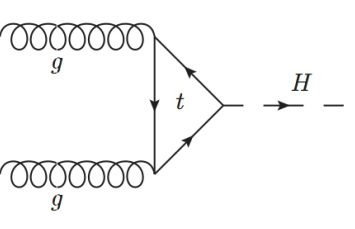
\includegraphics[width=1.5in]{images/ggf.png}
  \caption
   {The Feynman diagram for two gluons fusing into a Higgs. There are three vertices and this is a third order diagram. Two vertices involve the strong force and one vertex involves the Higgs coupling. The matrix element for this diagram would have two factors of the strong force coupling and one factor for the Higgs coupling which involves the mass of the top quark.}
  \label{fig:feynggf}
\end{figure}

%%%%%%%%%%%%%%%%%%%%%%%%%%%%%%%%%%%%%%%%%%%%%%%%%%%%%%%%%%%%%%%%%%%%%%%%%%%
\section{The Standard Model Higgs}


%%%%%%%%%%%%%%%%%%%%%%%%%%%%%%%%%%%%%%%%%%%%%%%%%%%%%%%%%%%%%%%%%%%%%%%%%%%
\subsection{SM Higgs Production and Decay Modes}

The SM Higgs can be created in a variety of ways. Some of these cross sections are shown below for 14 TeV collisions. The production cross sections are functions of the mass of the Higgs as well as the energy of the collisons. For a given collision energy the cross sections decrease as the Higgs mass increases: there are fewer kinematic possibilities for a heavier particle since more of the energy was used to create the particle. For a given mass, say 125 GeV, the cross section grows with collision energy. This constrasts with cross sections involving collisions of fundamental particles, e.g. electron antielectron collisions. This is an artifact of the fact that the LHC collides protons together. 

\begin{figure}[h!]
  \centering
  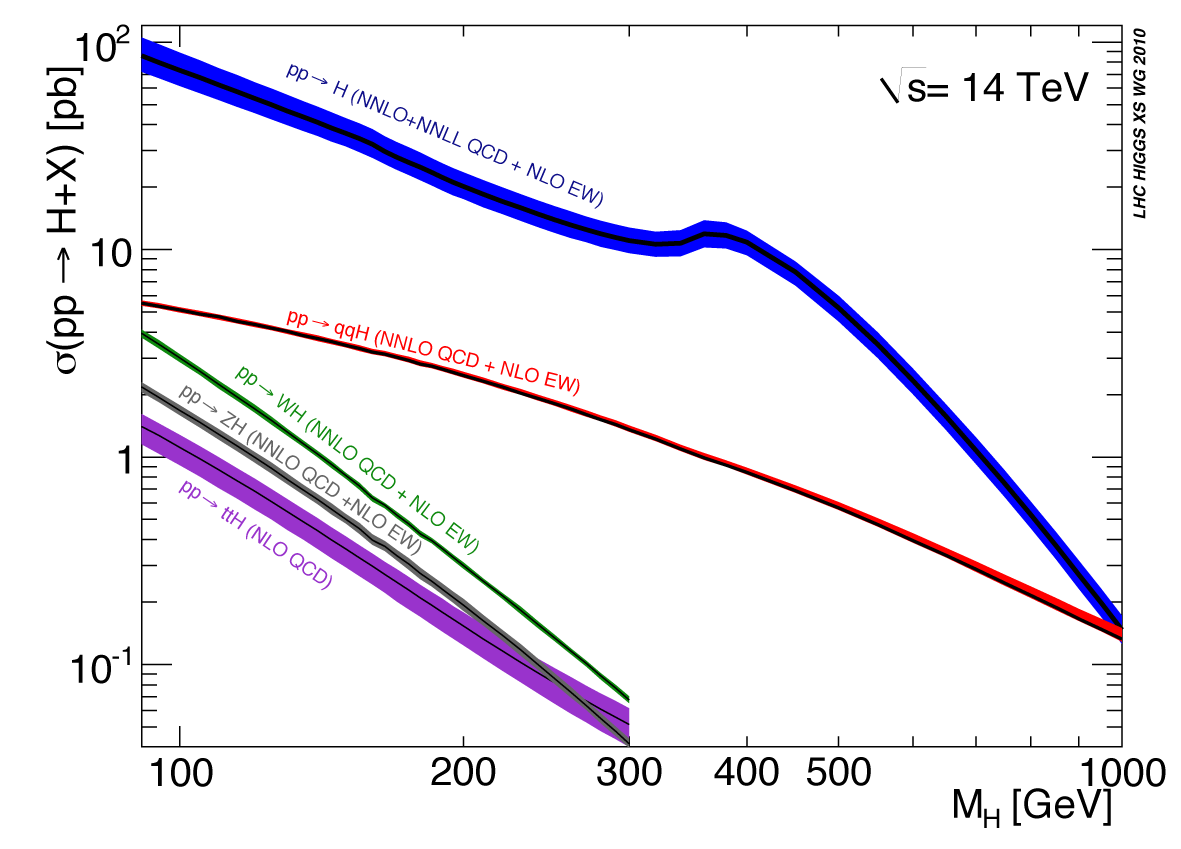
\includegraphics[width=5in]{images/14TeV_higgs_cross_sections.png}
  \caption
   {The highest production mode cross sections for the SM Higgs \cite{crossbranchplots}}
  \label{fig:hprodcross}
\end{figure}

Protons behave like a collection of an infinite number of quark-antiquarks, an infinite number of gluons, and the usual uud. The total momentum of the proton is divided up amongst them with lots of particles having little of the total momentum. The actual scattering events are between these more fundamental particles. The larger the total energy the smaller the fraction of energy needed to make a Higgs and since there are more particles with a lower fraction, this results in a growth of the cross section with collision energy. 

The SM Higgs is unstable and decays with a width of $\sim 5 MeV$ at 125 GeV. The probability of each decay changes depending upon the mass of the Higgs. In general the Higgs couples more strongly to particles with higher mass making the decays to heavier particles more likely.  

\begin{figure}[h!]
  \centering
  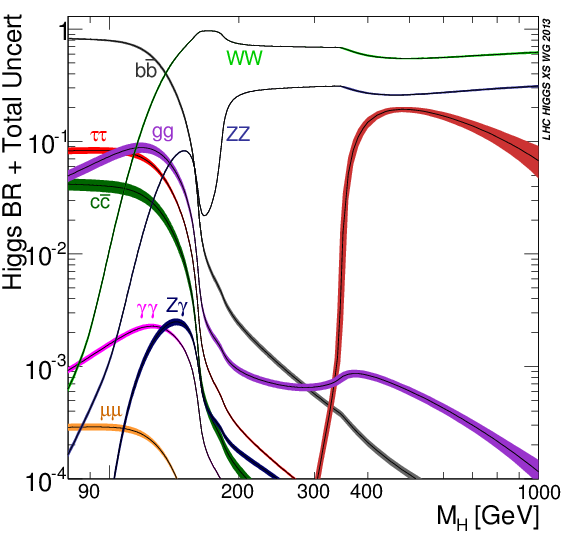
\includegraphics[width=3in]{images/Higgs_BR.png}
  \begin{tabular}{ |l|l| }
    \hline
    \multicolumn{2}{|c|}{Higgs Branching Ratios} \\
    \hline
    ${\rm b\tilde{b}}$ & 0.57 \\
    WW & 0.22\\
    gg & 0.085 \\
    ${\rm \tau\tau}$ & 0.065 \\
    ZZ & 0.027 \\
    ${\rm c\tilde{c}}$ & 0.027 \\
    ${\rm \gamma\gamma}$ & 0.0023 \\
    ${\rm Z}\gamma$ & 0.0016 \\
    ${\rm \mu^{+}\mu^{-}}$ & 0.00022 \\
    \hline
  \end{tabular} 
  \caption
{The graphic on the top left presents the SM Higgs branching fractions as functions of mass while the table on the bottom right displays the branching fractions for a 125 GeV SM Higgs \cite{crossbranchplots}.}
  \label{fig:hbranch}
\end{figure}

The muon has the lowest mass -- excluding the photon and gluon -- of the particles in Figure ~\ref{fig:hbranch} and consequently H$\rightarrow \mu^{+}\mu^{-}$ has the lowest branching fraction in the set. \footnote{The Higgs also couples to the electron and the first generation quarks but the masses are so light that CMS does not expect to see the SM Higgs in those modes.} The gluons and photons are massless and do not couple to the Higgs at leading order. These massless vector bosons interact with the Higgs through a loop of top quarks. The extremely heavy mass of the top quark, about 173 GeV, balances the fact that the loop production is a higher order mechanism.  
\begin{figure}[h!]
  \centering
  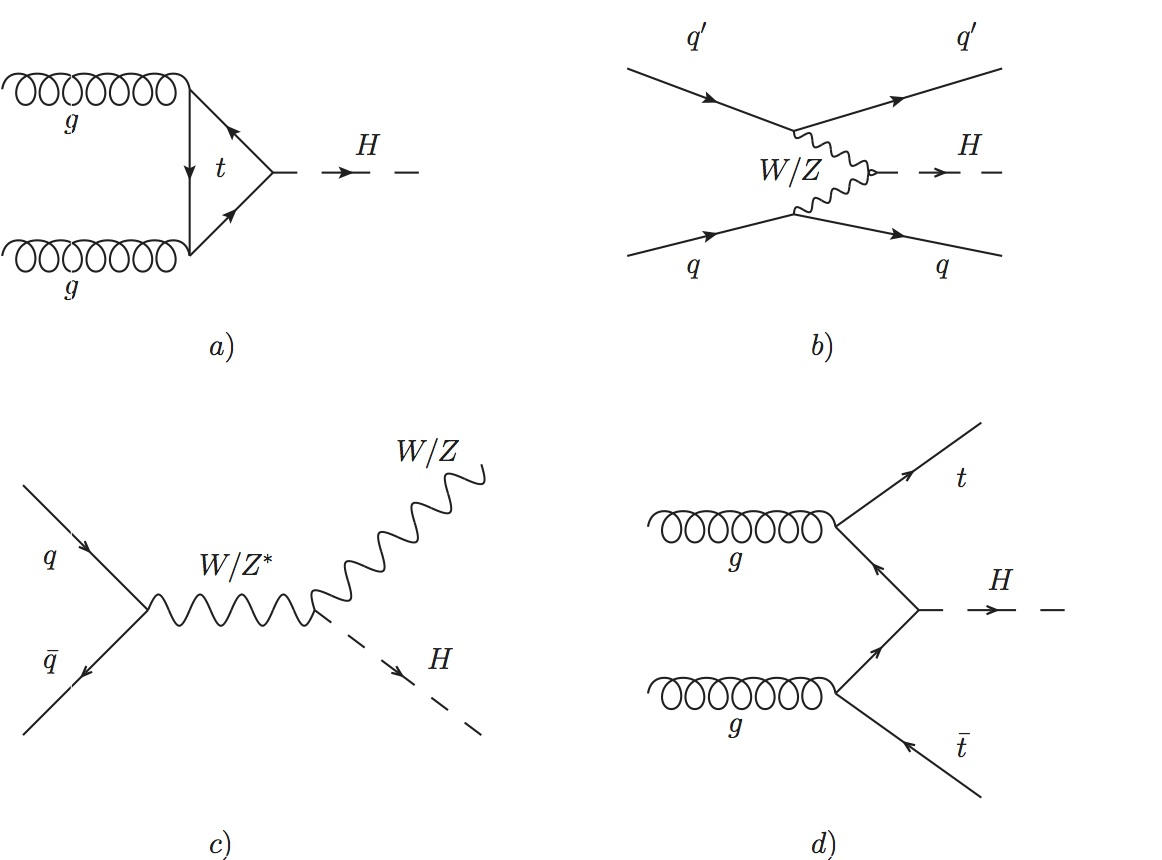
\includegraphics[width=4in]{images/higgs_production_modes.png}
  \caption
   {The SM production modes with the highest cross sections. a) Gluon Gluon Fusion (GF) b) Vector Boson Fusion (VBF) c) Associated Production with a Vector Boson (VH) d) ${\rm t\tilde{t}}$H}
  \label{fig:hfeynprod}
\end{figure}

The Higgs to massless vector boson coupling via the top loop is seen in the GF Feynman diagram in Figure ~\ref{fig:hfeynprod}. At ${\rm M_{h} = 125}$ GeV, ${\rm \sqrt{s} =}$ 13 TeV, the GF channel comprises 87\% of the total Higgs production cross section, VBF 7\%, VH 4\%, and ${\rm t\tilde{t}}$H 1\% \cite{crossbranchplots}. Besides ${\rm t\tilde{t}}$H, the process q + $\tilde{q} \rightarrow$ H isn't considered due to its low cross section. The low masses of the other quarks suppress the process. 

Quark gluon (qg) scattering is a major background for the Higgs to two jets decays since the process closely resembles GF in this mode.   

\begin{figure}[h!]
  \centering
  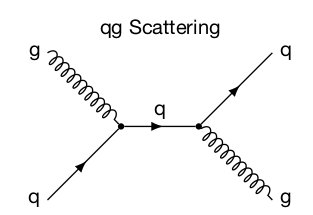
\includegraphics[width=2in]{images/qg_scattering.png}
  \caption
   {Quark gluon scattering creates many two jet events. This background looks very similar to GF when the Higgs decays to two jets. The colliding protons are made of quarks and gluons so this process is extremely common.}
  \label{fig:feynqg}
\end{figure}

